\chapter{Event Selection}\label{selection}

The data used in this analysis was collected online using a trigger designed to record events that
contain large values of $\HT^{\text{miss}}$ and $\MET$. The details of the trigger were explained in the chapter \ref{samples}. Offline, all events are required to have at least one primary vertex reconstructed within a 24 cm window along the beam axis, with a transverse distance from the nominal pp interaction region of less than 2 cm. In the presence of more than one vertex passing these requirements, the primary-event vertex is chosen to be the one with the highest total $\pt^{2}$, summed over all the associated tracks.

In the signal region we select events that contain highly energetic AK8 jets and large missing transverse energy.
An event falls into this category if the AK8 jets have $\pt >$ 200 GeV, $\left| \eta\right| <$ 2.4, $65\leq  m_{\text{jet}} \leq105$ GeV and $\tau_{21}<0.75$. For the missing energy, we require $\MET> 250$ GeV. If the selected event contains more than one AK8 jet with the previous requirements, the jet with the largest $\pt$ is chosen in order to calculate the transverse mass variable.
Also, a lower threshold of 600 GeV in the transverse mass is required in the selected events. Below this value, a new resonance would not be massive enough to produce a large fraction of boosted V bosons, resulting in a low value of the selection efficiency.

Background from leptonic W boson decays is reduced through rejection of events with isolated leptons (electrons, muons, taus) identified with loose selection criteria. Events containing b-jets are vetoed in the analysis in order to suppress $t\bar{t}$ background. Events containing identified photons are reject to reduce V +$\gamma$+jets backgrounds. To supress QCD multijet background in which large $\MET$ could arise,
the minimum azimuthal angle between the $\MET$ direction and the AK4 jets with $\pt$ greater than 30 GeV is required to be greater than 0.5. 
Table \ref{tab:finalsel} summarize the final selection chosen in the analysis.

In order to set object disambiguation between possible VZ candidates, we use as a selection criteria the candidate with the highest transverse momentum in the event.

The signal efficiency in each category ($\varepsilon_{\text{cat}}$) is defined as the ratio between the number of signal events after the hole analysis selection in a chosen category ($N^{\text{cat}}_{\text{sel}}$) over the total number of generated signal events ($N_{\text{gen}}$).

\begin{eqnarray}
\varepsilon_{\text{cat}} = \dfrac{N^{\text{cat}}_{\text{sel}} }{N_{\text{gen}}},\qquad  \text{cat = HP,LP} 
\end{eqnarray}

The signal efficiencies are evaluated for the full analysis selection inside the VZ-enriched ($65 \leq  m_{\text{jet}} \leq 105$ GeV) mass windows, and are shown in figure \ref{fig:eff} for the bulk graviton signal model for several mass points and different categories. The high purity efficiency drops at high values of the resonance mass due to the inefficiency of the N-subjettines and jet mass selection; this is partially recovered in the low purity category.

Figure \ref{fig:controlplots1} shows a set of comparison plots between data and simulation for interesting variables in the analysis. The final analisys selection except for a loose requirement in the mass of the jet $40 \leq  m_{\text{jet}} \leq 220$ GeV was used to produce the plots in order to observe regions that will be employed for background estimation (sideband regions). In general a good agreement between data and simulation is observed in the control plots.

\def\arraystretch{1.2}
\begin{table}[h]
\begin{footnotesize}
\caption{Final analysis selection.}
\label{tab:finalsel}
\begin{tabular}{|c|cc|}
\hline
\textbf{Selection}                     &                                       &       \textbf{Value}                                                   \\  \hline
High Level Trigger                     &                                       &      $\verb|PFMETNoMu90_JetIDCleaned_PFMHTNoMu90_IDTight|$      \\ 
                                       &                                       &       OR $\verb|HLT_PFMET170_*|$                               \\ \hline
                                       &                                       &      Type-I PF MET                                            \\      
\raisebox{1.5ex}[0pt]{$E_{\text{T}}^{\text{miss}}$} &                          &      $p_{T} > 250$ GeV                                        \\ \cline{1-3}
                                       &                                       &      PFJetID Loose                                            \\  
                                       &                                       &      $p_{T} > 200$ GeV, $\left|\eta\right|< 2.4$               \\  
                                       & \raisebox{1.5ex}[0pt]{AK8Jets}              &      $ 65 < m^{\text{pruned}}_{\text{jet}} < 105$ GeV           \\  
\raisebox{1.5ex}[0pt]{Jets}            &                                       &      CHF $> 0.1$, NHF $< 0.8$                                   \\  \cline{2-3}
                                       &                                       &      PFJetID Loose                                            \\  
                                       &                                       &      $p_{T} > 30$ GeV, $\left|\eta\right|< 2.4$               \\  
                                       &  \raisebox{1.5ex}[0pt]{AK4Jets}       &      CHF $> 0.1$, NHF $< 0.8$        \\
                                       
                                       &                                       &      $\text{min}\Delta \phi(\text{AK4Jet},\MET) >$ 0.5             \\
                                       &                                       &      b-tag Veto : CSV $>$ 0.8 
 
                           \\  \cline{1-3}
Leptons (electrons, muons, taus)                                &                                       &      Veto                                                        \\  \cline{1-3}
Photons                                &                                       &      Veto                                                      \\ \cline{1-3}
VZ candidate transverse mass           &                                       &      $M^{\text{T}}_{\text{VZ}} > 600$ GeV                      \\ \cline{1-3}
\end{tabular}
\end{footnotesize} 
\end{table}

\begin{figure}[!ht]
\caption{ Signal efficiency for $G_{Bulk} \rightarrow ZZ \rightarrow $ jet + $\MET$ for different mass points and different categories after the final analysis selection.}
\begin{center}
  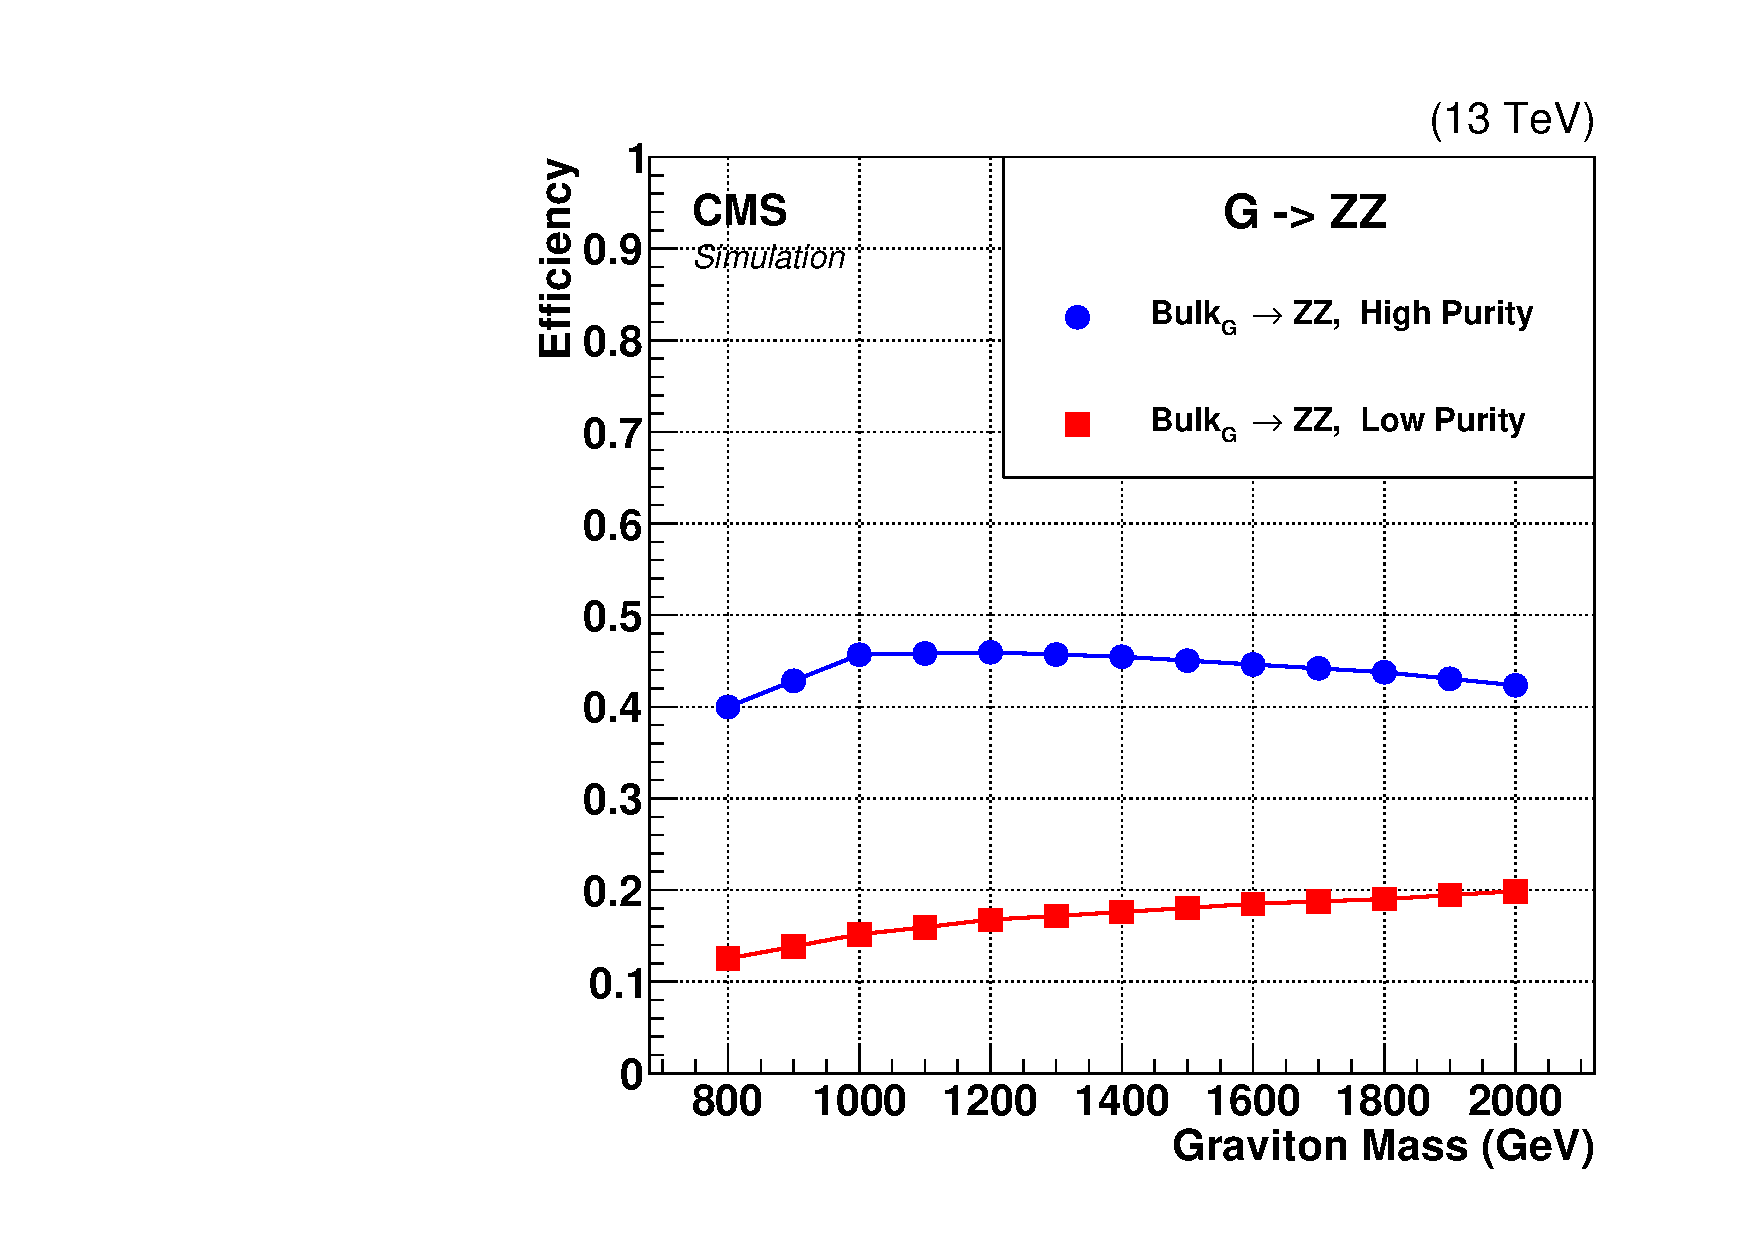
\includegraphics[width=280pt]{figuresARC/sigeff/efficiency.pdf}
\end{center}
\label{fig:eff}
\end{figure}



\begin{figure}[!ht]
\caption{Top:(left) AK8 Jet transverse momentum. (right) Missing transverse energy. Center: (left) AK8 Jet pseudorapidity. (right) min $\Delta \phi$ distribution. Bottom: (left) Pruned jet mass. (right) Candidate transverse mass. The plots show the comparison between data(black dots) and simulation. The simulation is composed by different backgrounds: Z+jets(light yellow), W+jets(orange), $t\bar{t}$(green), QCD multijets(light blue) and diboson(light pink). The statistical uncertainty is shown in dark pink. In addition a Bulk graviton signal sample of 1.2 TeV is shown by the orange hatch region. The figure also show the ratio of the histograms (data/simulation) and the $\chi^{2}/\text{ndf}$ value as a figure of merit.}
\begin{tabular}{cc}
  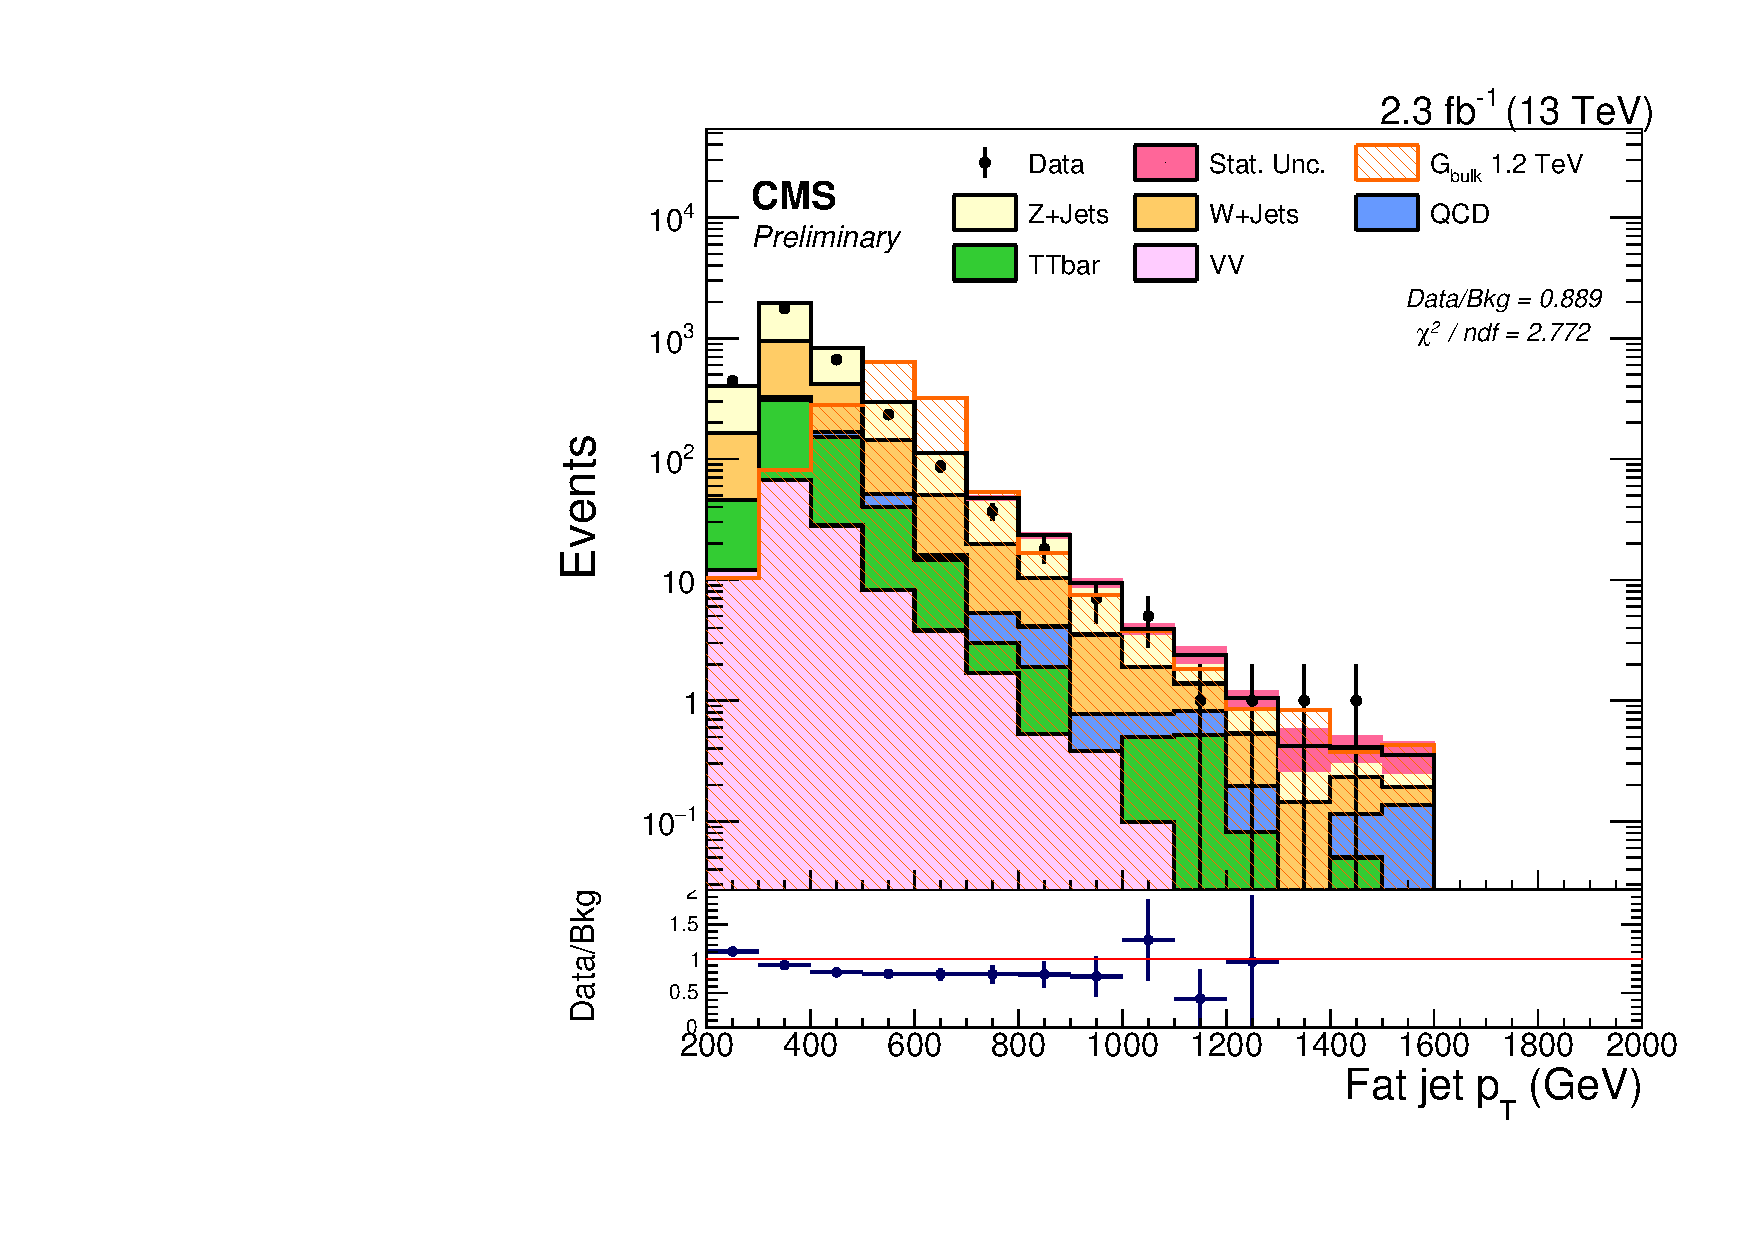
\includegraphics[width=180pt]{Chapter6_plots/LOG_can_h_ptZjj.pdf} &
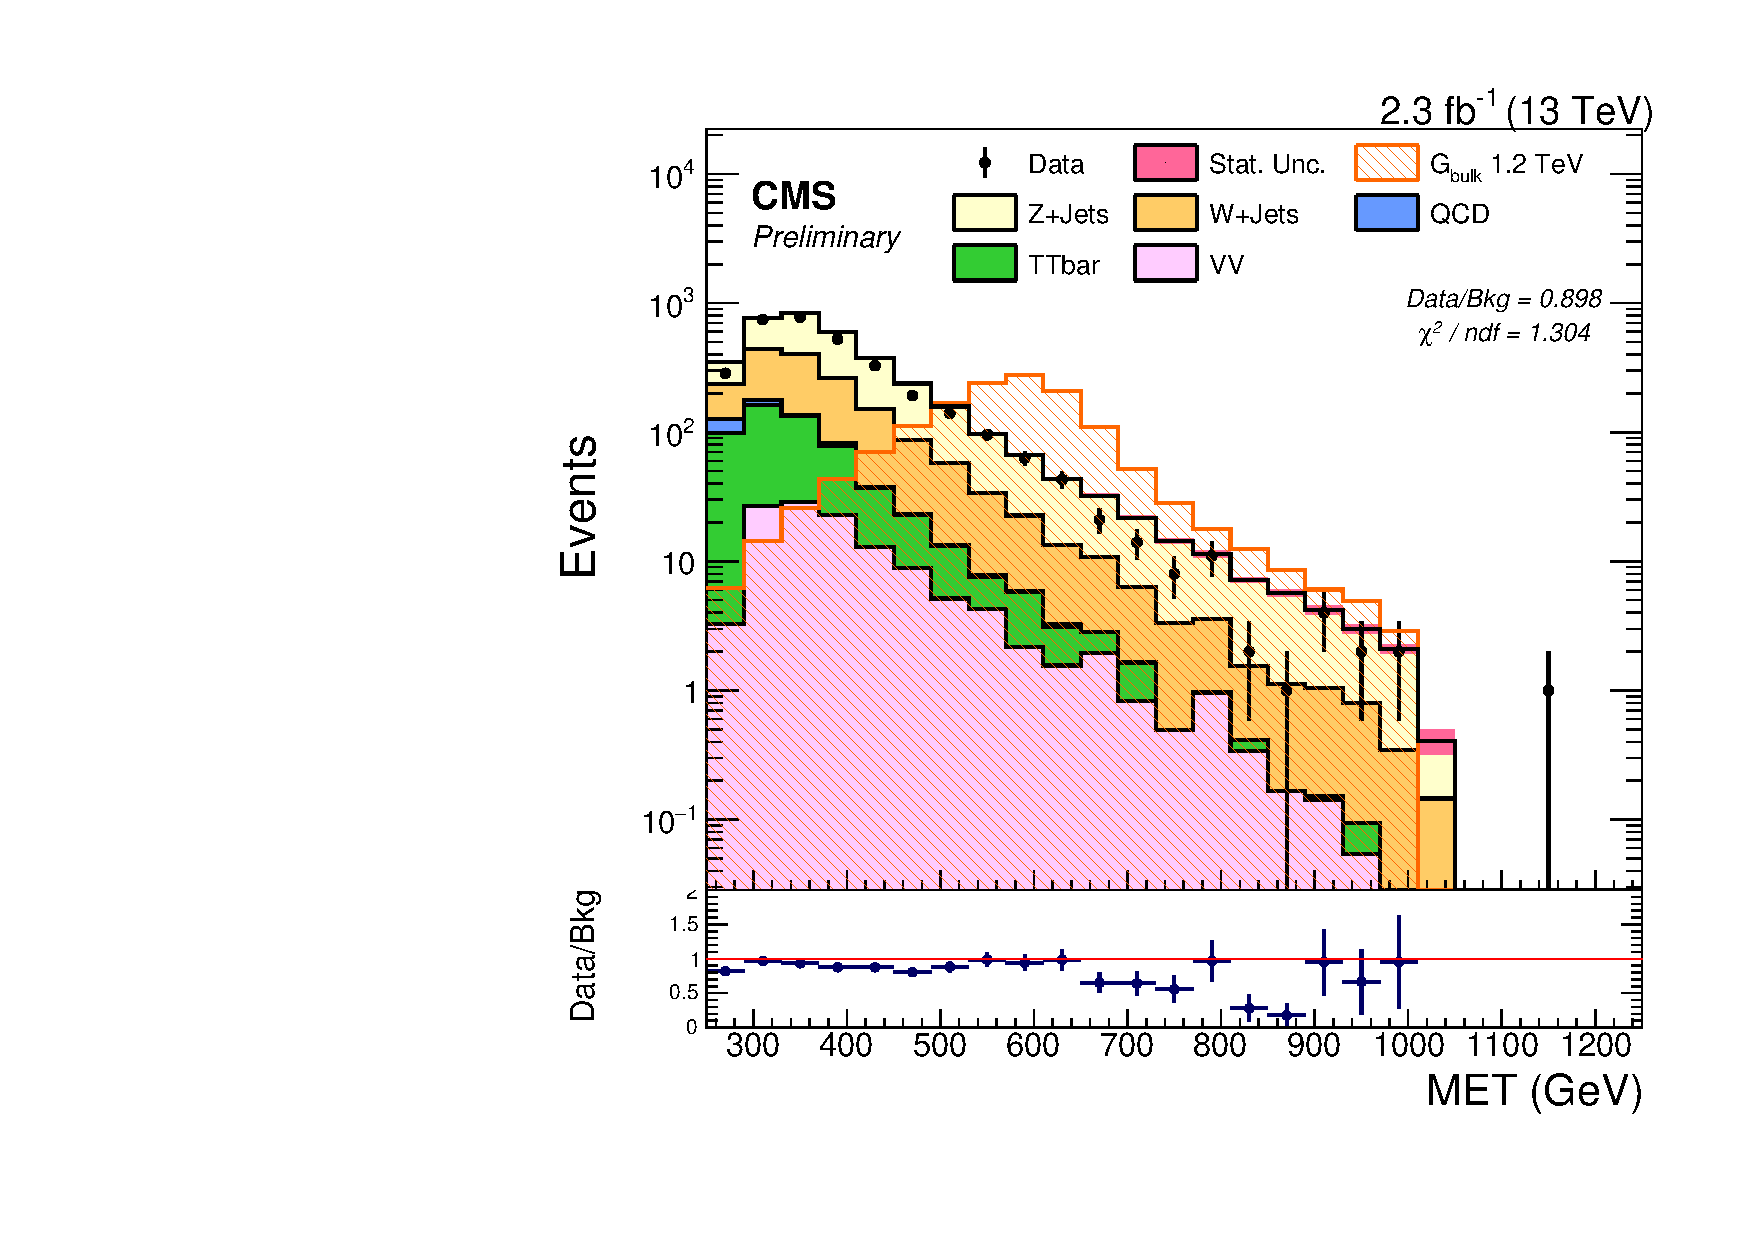
\includegraphics[width=180pt]{Chapter6_plots/LOG_can_h_metpt.pdf}\\
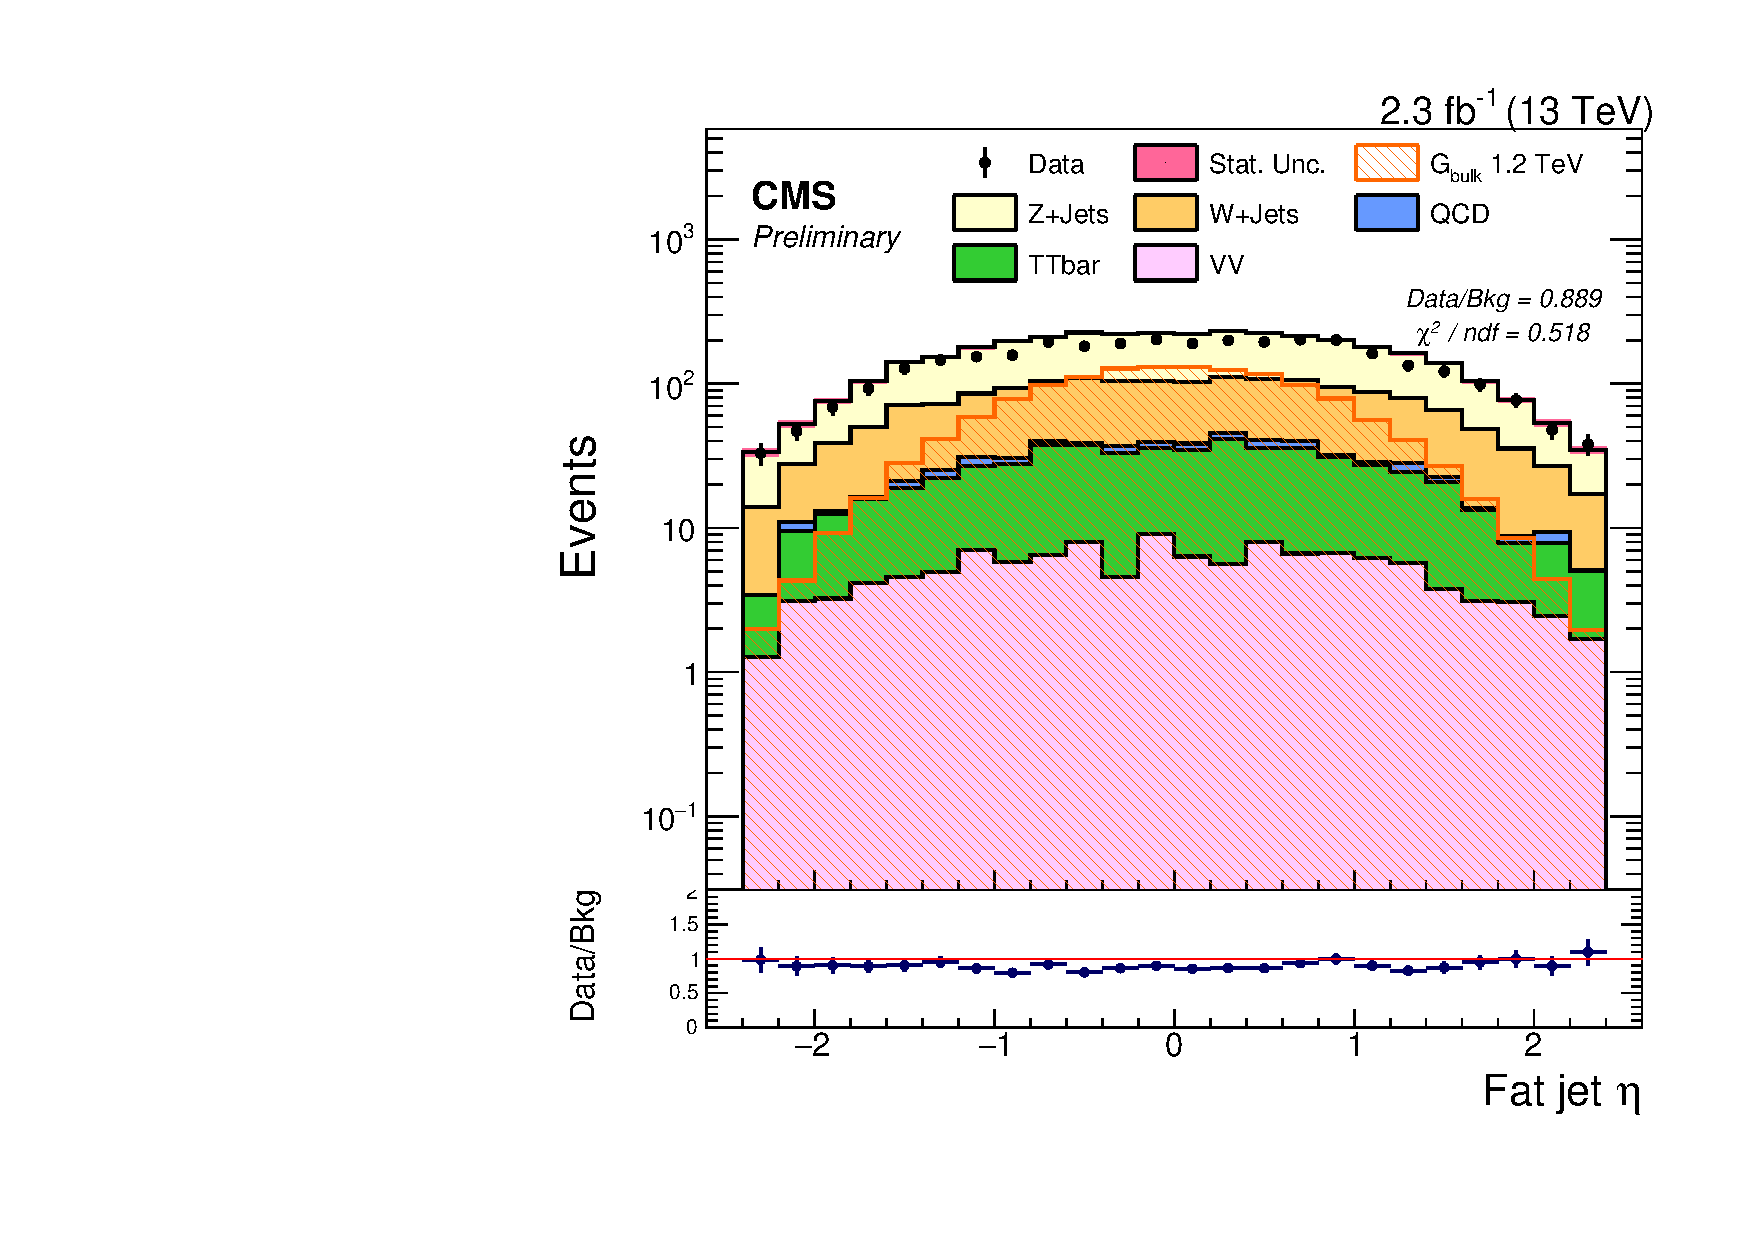
\includegraphics[width=180pt]{Chapter6_plots/LOG_can_h_yZjj.pdf} &
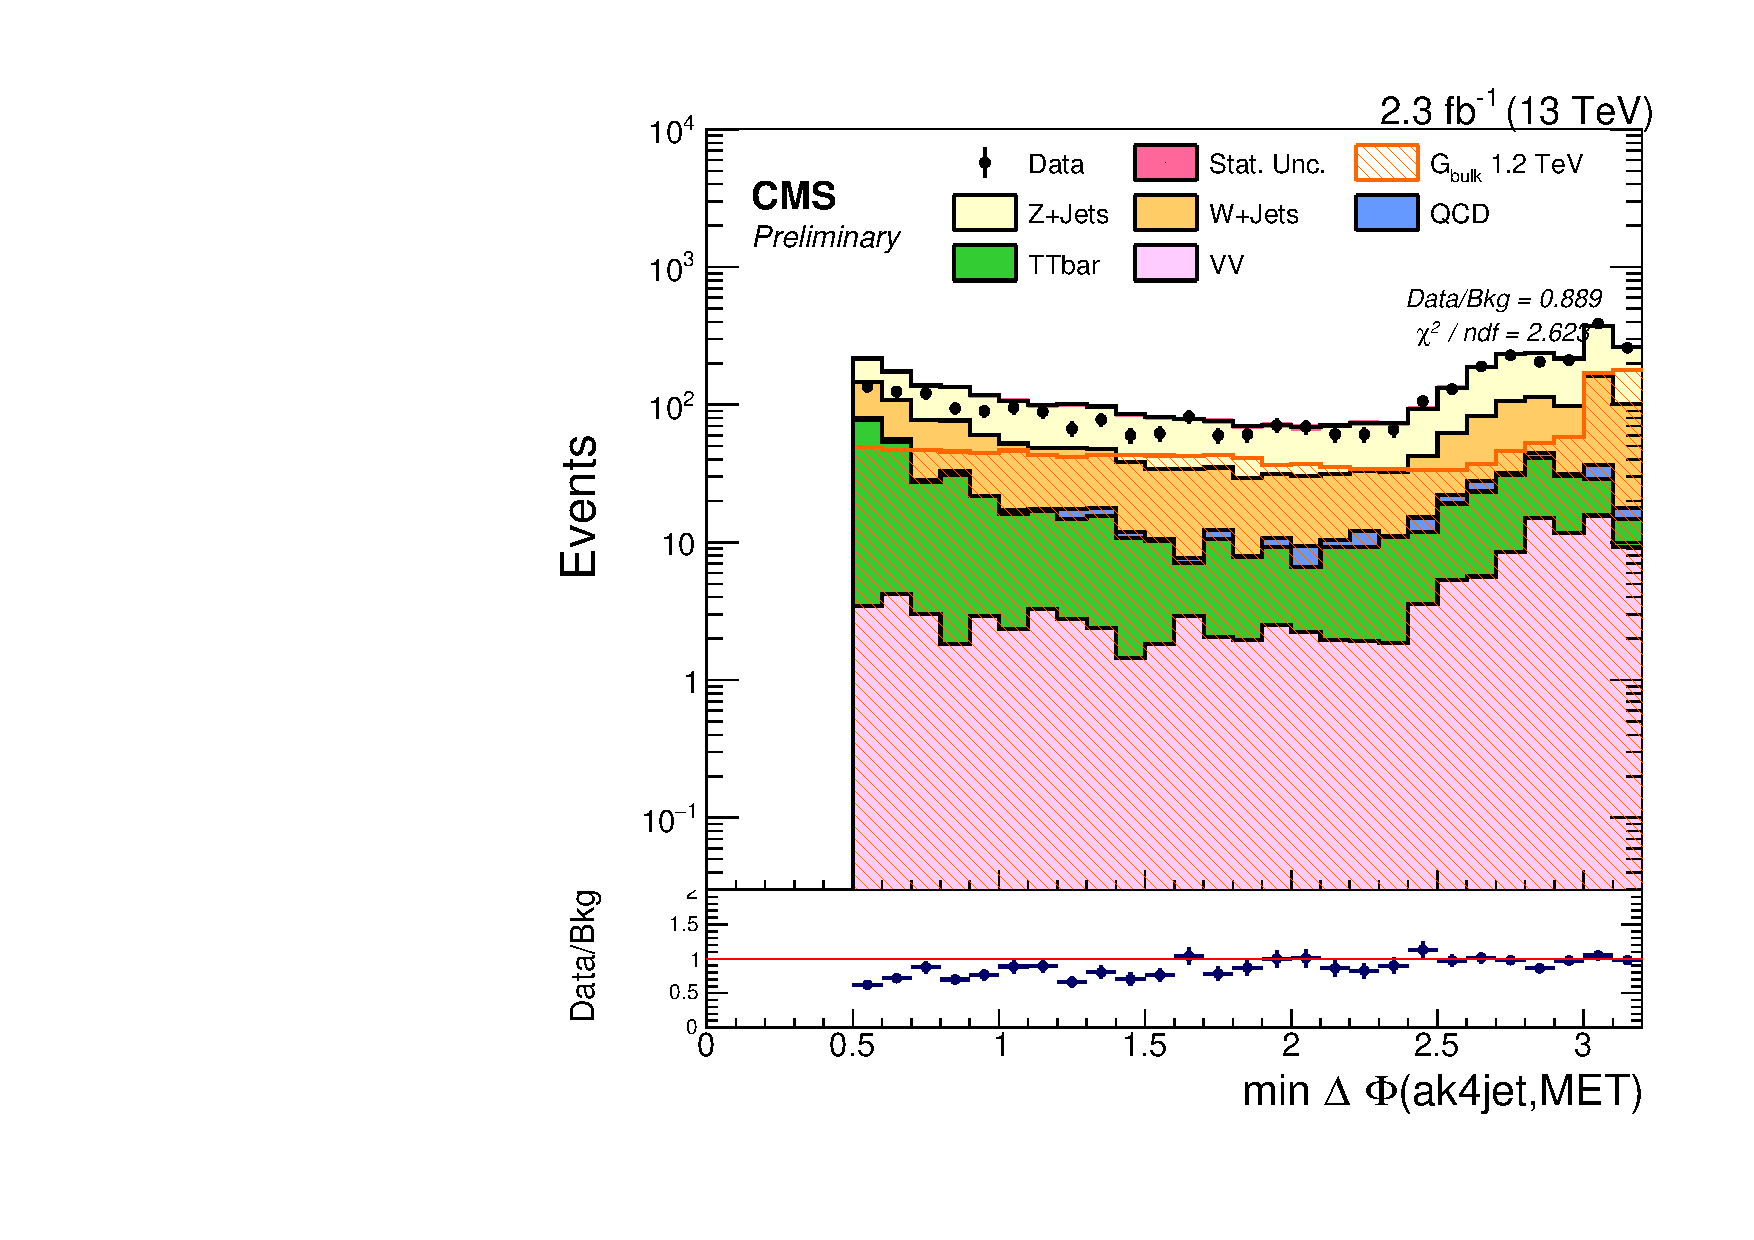
\includegraphics[width=180pt]{Chapter6_plots/LOG_can_h_minabsdeltaphi.pdf}\\
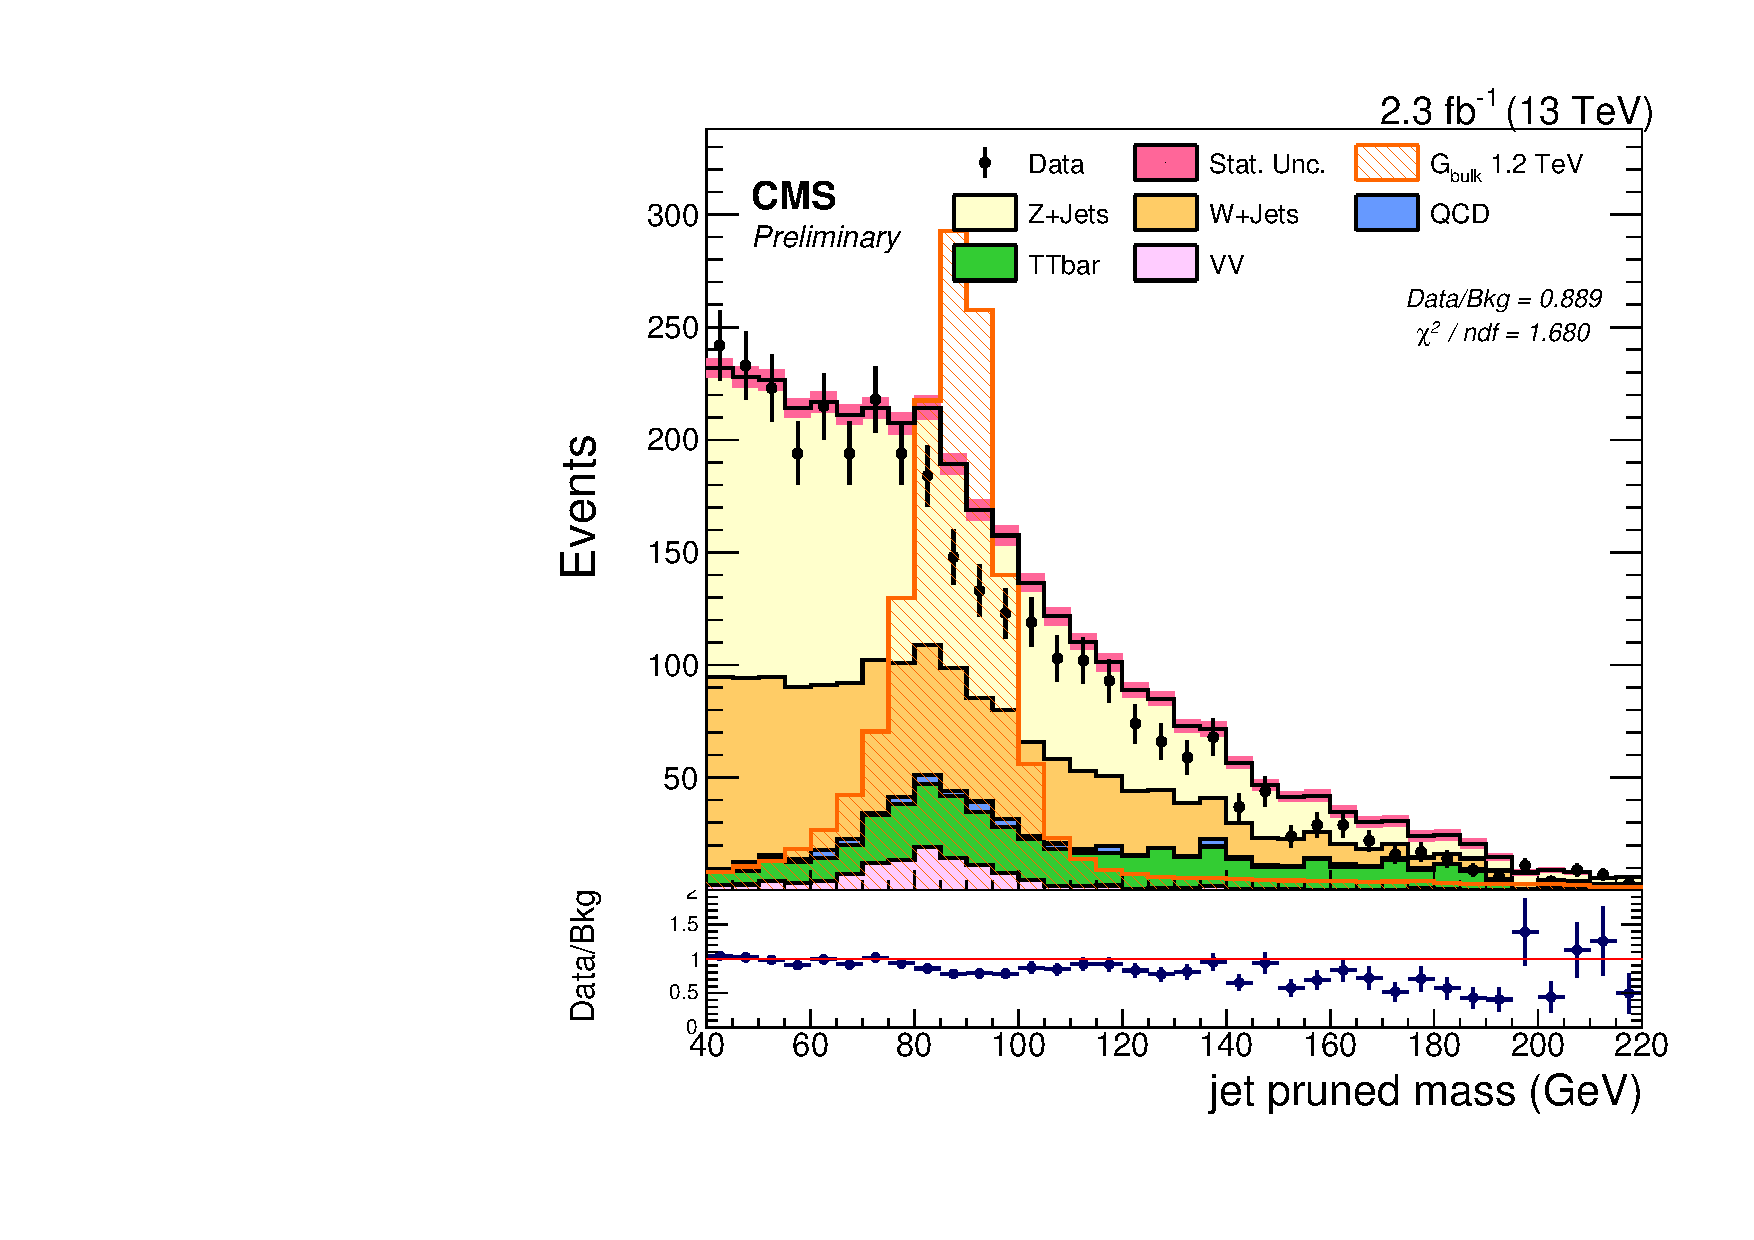
\includegraphics[width=180pt]{Chapter6_plots/can_h_massZjj.pdf} &
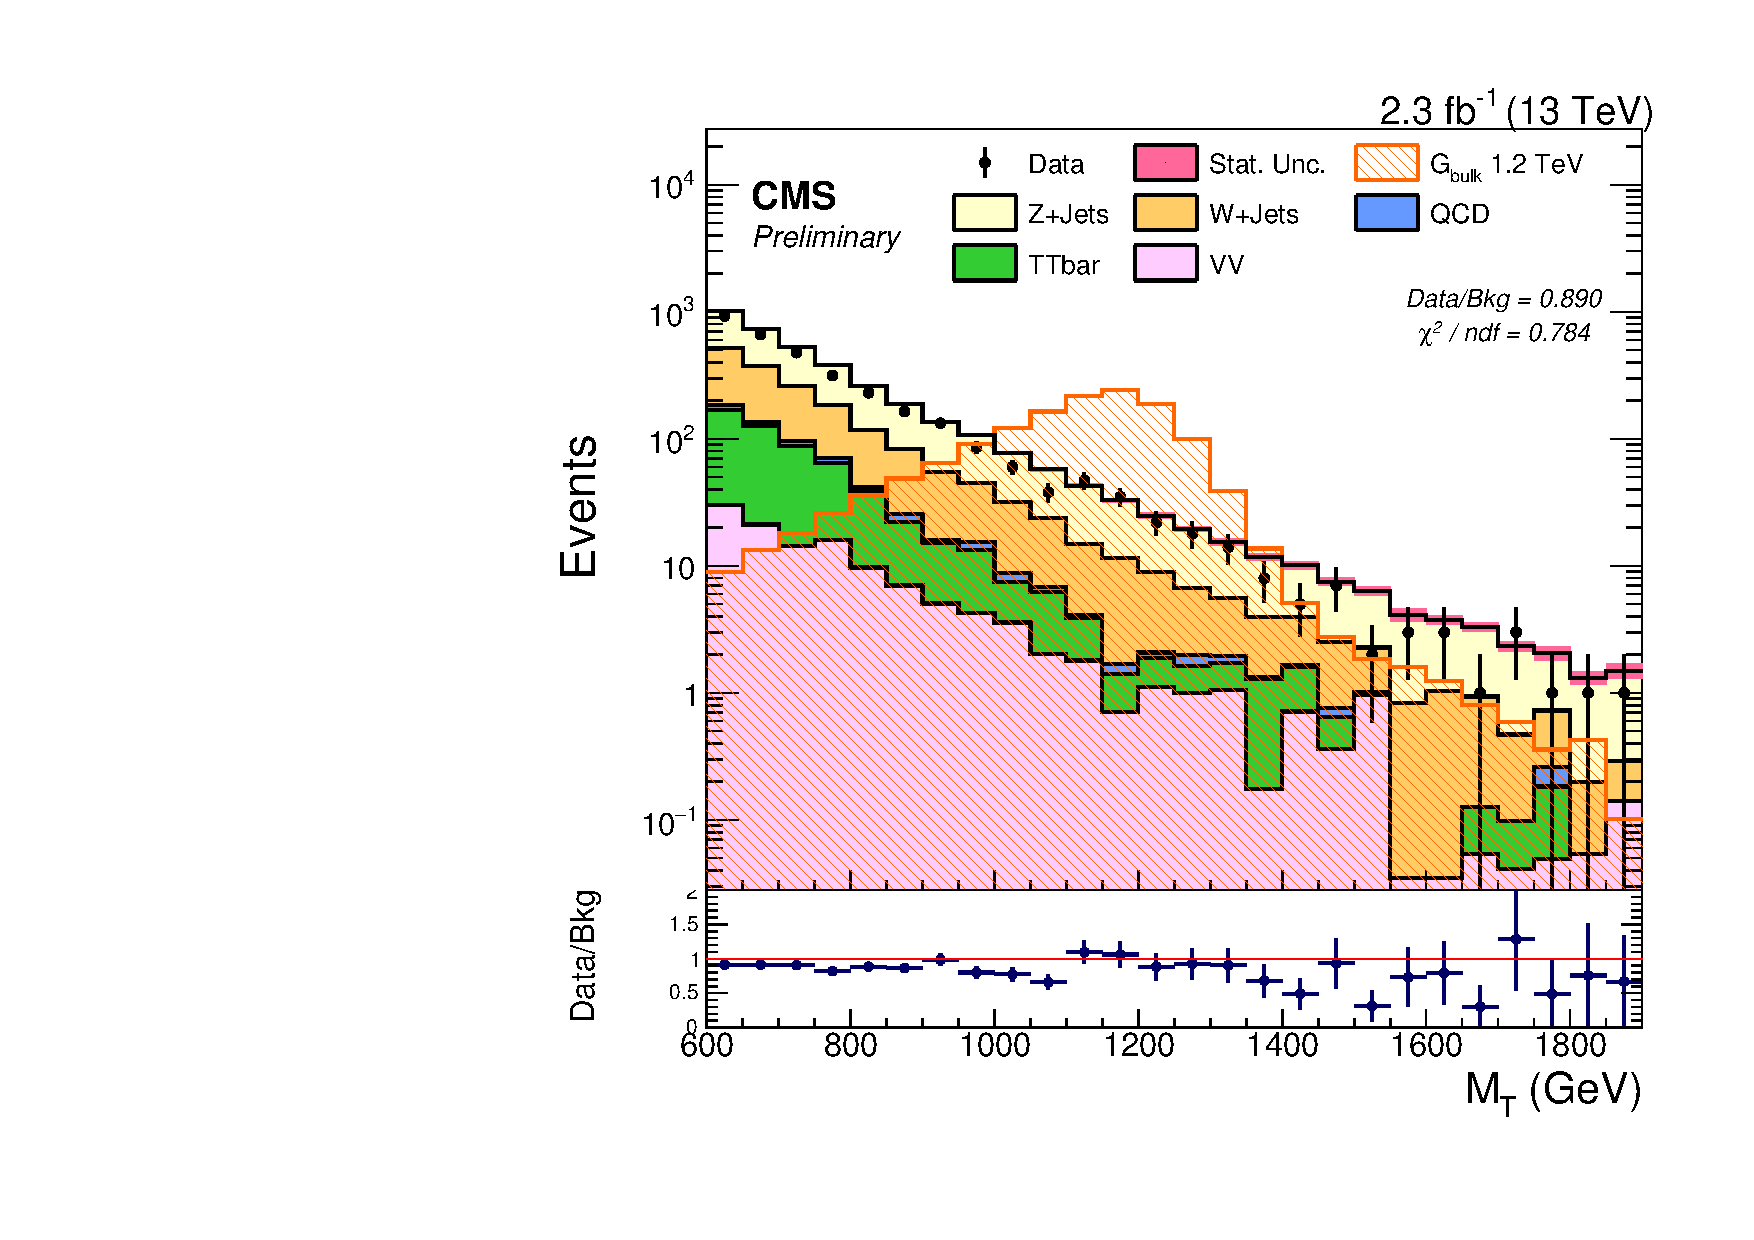
\includegraphics[width=180pt]{Chapter6_plots/LOG_can_h_candTMass.pdf}\\
\end{tabular}
\label{fig:controlplots1}
\end{figure}